% rad.tex

\documentclass{report}
\linespread{1.2}
\renewcommand{\chaptername}{}
\usepackage{times} %Times is nice
\usepackage{url}
\usepackage[T1]{fontenc}
\usepackage{titlesec, blindtext, color}
\usepackage{amsmath}
\usepackage{graphicx}
\usepackage{hyperref}
\usepackage{float}

\definecolor{gray75}{gray}{0.75}
\newcommand{\hsp}{\hspace{20pt}}
\titleformat{\chapter}[hang]{\Huge\bfseries}{\thechapter\hsp\textcolor{gray75}{|}\hsp}{0pt}{\Huge\bfseries}

\begin{document}

\title{Requirements and Analysis Document (RAD) for Barcode Scanner Project - Group 30}
\author{
    Christian Svensson\\
    \and
    Olle Andreasson\\
    \and
    Olof Karlsson\\
    \and
    Rasmus Letterkrantz
}
\date{\today}
\maketitle

\tableofcontents

\chapter{Introduction}

The Barcode Scanner is an android application that is meant to be used by small-time shop owners, potentially replacing conventional barcode scanners. Since most people own a smartphone, we believe this could also be useful for anyone wanting to keep track of items that carry conventional barcodes, and store them in a database.

\section{Purpose of Application}
The project aims towards creating an application for scanning and analyzing barcodes with android devices.

\section{General Characteristics of Application}
The application will be an Android application with a graphical user interface. It will take use of the camera to take snapshots. Once the application have an image containing a barcode, it will be analyzed to generate an identification number. This will be compared to a database to result in a product as output.\cite{website:barcodescanner}

\section{Scope of Application}
The application will not be guaranteed to work on every android platform, it will be tested on version 4.1.1 and this will be the only version that is guaranteed to work. The application will not necessarily generate standard barcode ids.

\section{Objectives and Success Criteria of the Project}

\begin{enumerate}
  \item The application will be able to take a picture using the back-facing camera on your phone.
  \item The application will then scan that image for a possible barcode.
  \item The application will be able to generate a unique id from that barcode.
  \item The application will be able when given an id, compare it to the database content, and if the id exists, return a product.
\end{enumerate}

\section{Definitions, Acronyms and Abbreviations}

\begin{itemize}
    \item{GUI}, Graphical User Interface.
    \item{Android}, open source operating system for mobile units (smart-phones, tablets, etc).
    \item{Java}, platform independent programming language.
    \item{XML}, Extensible Markup Language is used for structuring the elements in the GUI.
    \item{SQLite}, the database used to store the barcodes.
    \item{Locator}, class used to locate the barcode on a given image.
    \item{Generator}, class used for analyzing the pattern extracted by the Locator and generating the actual key.
    \item{MVC}, a way of partition an application with a GUI into distinct parts avoiding a mixture of GUI-code, application code and data spread all over.
    \item{ADT}, the Java Runtime Environment. Additional software needed to run an Java application.
    \item{.apk}, application package file, a file format use to distribute and install application software and middleware onto Android.
\end{itemize}

\chapter{Requirements}

\section{Functional Requirements}

\begin{enumerate}
  \item Take a picture.
  \item Scan the picture for any barcode (parse).
  \item Match (read) or add (write) any result to a database.
  \item End the application (turn of camera and exit the process).
\end{enumerate}

\section{Non-Functional Requirements}

\subsection{Usability}
Aim for simplicity! The application should be simple to use, the GUI should be clean and the flow should be straightforward for any user. The scanner should pass tests from users who are not, by any means, an advanced android user.

\subsection{Reliability}
Each combination of numbers that we generate from each barcode should match the general combination that the barcode represents (as long as the barcode is in the correct EAN format).

\subsection{Supportability}
The application Gui should be clean and scalable with the screen size of the given device.
There should be automated test verifying most use cases. Code related to the GUI could be tested manually. GUI test should be recorded and included in the final documentation.

\subsection{Performance}
The scanning should be quite fast and the application should not weigh down the time for the camera to take and present a picture.

\subsection{Implementation}
The application should be using the standard Android-specific Java environment.

\subsection{Packaging and installation}
Installation should be done using a standard .apk file containing the application, that the user can then install on their Android device.

\subsection{Legal}
Android is a open platform, freely available to developers everywhere. The barcode standard our algorithm will detect is EAN-13, which is an international standard freely available.

\pagebreak

\chapter{Application models}
This is the UML diagram for the project:
\begin{figure}[H]
		\centering
		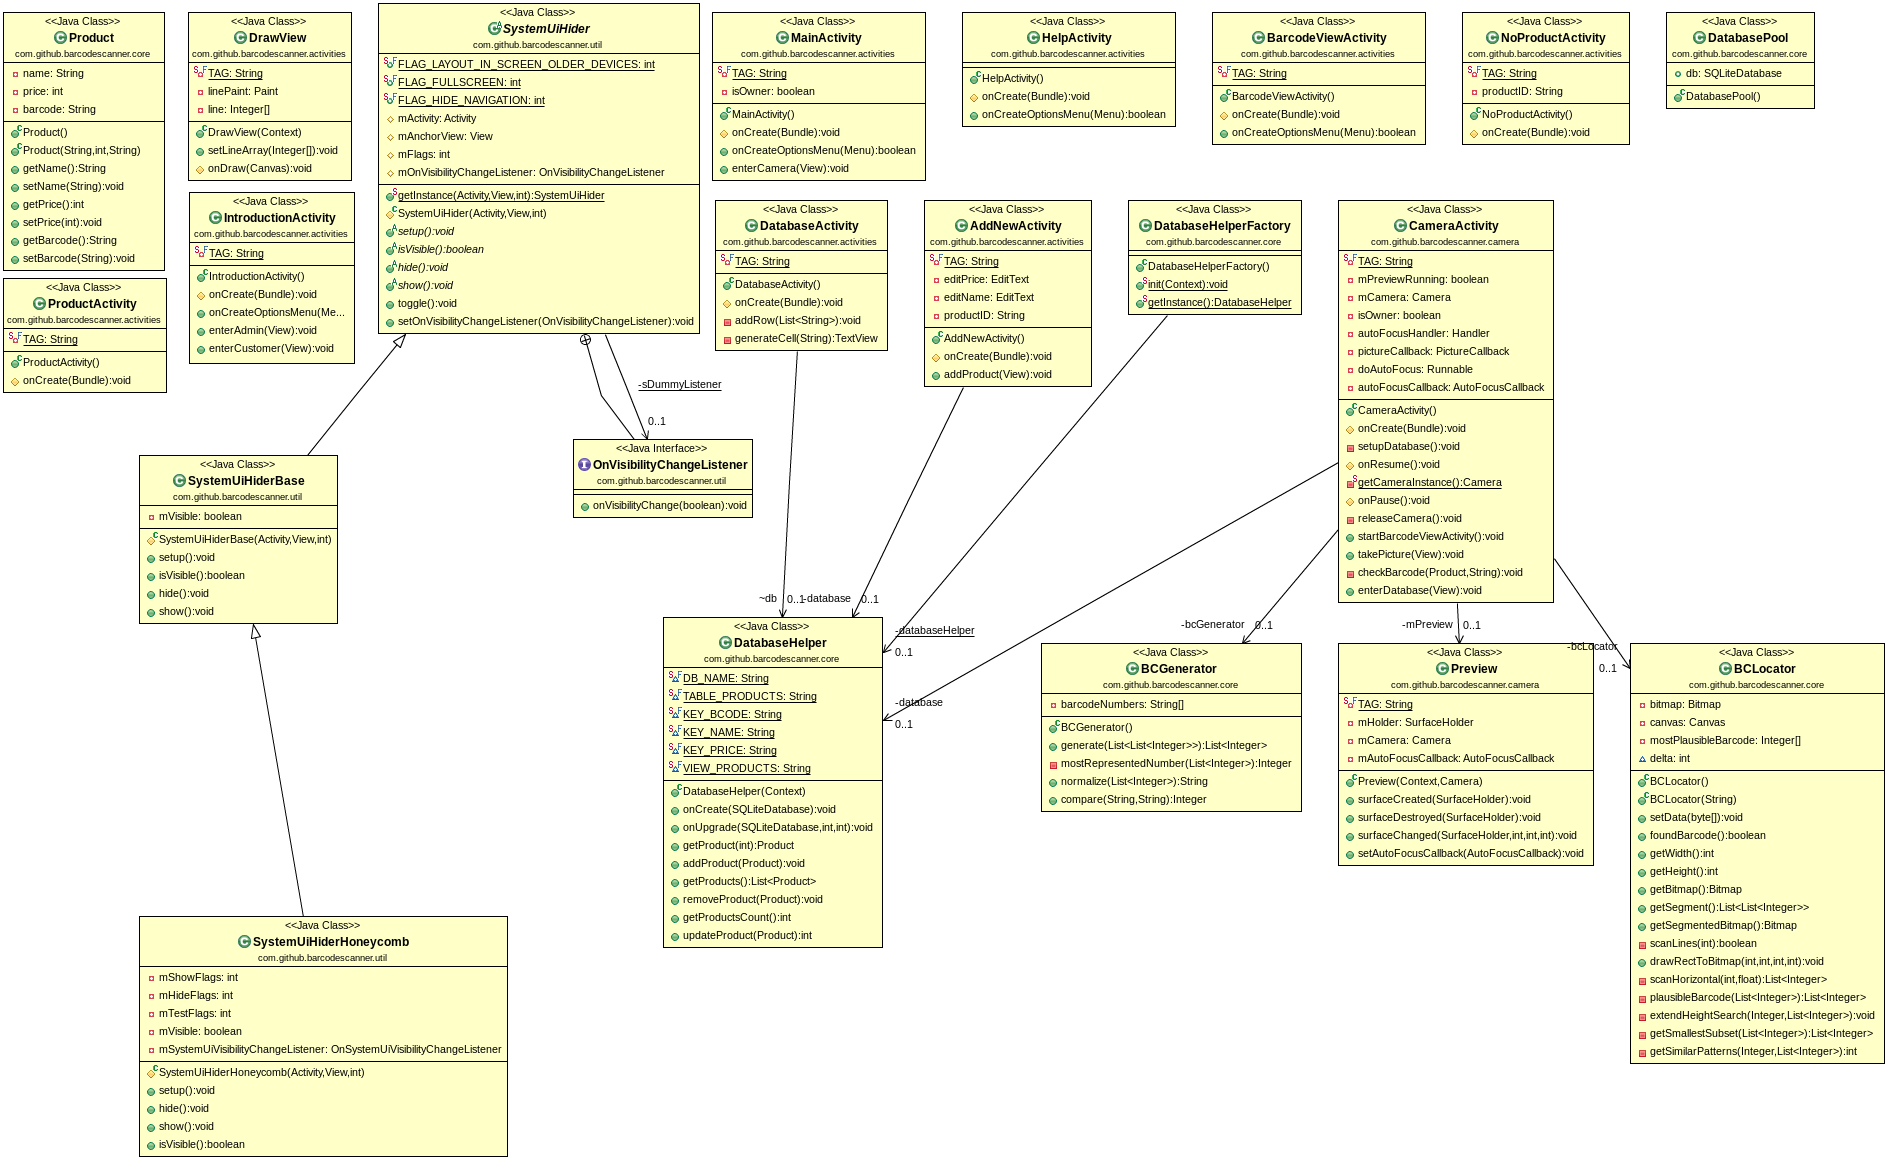
\includegraphics[width=\textwidth]{uml.png}
		\caption{UML}
		\label{fig:UML}
\end{figure}



\subsection{Use cases}
Here follows the use cases for the barcode scanner project, in order of priority: 

\begin{enumerate}

  \item Scan an image containing a new barcode. \

    \textbf{Summary:} This is how the user actually scans a barcode. \\
    \textbf{Priority:} High \\
    \textbf{Extends:} - \\
    \textbf{Includes:} - \\
    \textbf{Participators:} Actual user \\
    \textbf{Normal flow of events} \\
    \textbf{Flow 1} \\ A barcode is found in the image. \\

    \begin{tabular}{ | p{1cm} | p{3cm} | p{4cm} |}
    \hline
      & Actor & System \\ \hline
    1.1 & Clicks the "Scan" button & \\ \hline
    1.2 & & Displays a view where the user is prompted to input a name and a price for the scanned barcode. \\
    \hline
    \end{tabular} \\

    \textbf{Alternate flow} \\
    \textbf{Flow 2} \\ No barcode is found in the image. \\

    \begin{tabular}{ | p{1cm} | p{3cm} | p{4cm} |}
    \hline
      & Actor & System \\ \hline
    2.1 & & Nothing happens. \\
    \hline
    \end{tabular} \\

    \textbf{Exceptional flow} \\ There is no exceptional flow.

  \item Save a scanned barcode into the database as a new product. \

  \item Find a scanned barcode in the database. \

    \textbf{Summary:} This is how the user scans a barcode that already exists in the database. \\
    \textbf{Priority:} High \\
    \textbf{Extends:} Use Case 1 \\
    \textbf{Includes:} - \\
    \textbf{Participators:} Actual user \\
    \textbf{Normal flow of events} \\
    \textbf{Flow 1} \\ A barcode is found in the image. \\

    \begin{tabular}{ | p{1cm} | p{3cm} | p{4cm} |}
    \hline
      & Actor & System \\ \hline
    1.1 & Clicks the "Scan" button & \\ \hline
    1.2 & & Displays a view where the user can view the information that the database stores about the matching barcode. \\
    \hline
    \end{tabular} \\

    \textbf{Alternate flow} \\
    \textbf{Flow 2} \\ No barcode is found in the image. \\

    \begin{tabular}{ | p{1cm} | p{3cm} | p{4cm} |}
    \hline
      & Actor & System \\ \hline
    2.1 & & Nothing happens. \\
    \hline
    \end{tabular} \\

    \textbf{Exceptional flow} \\ There is no exceptional flow.

  \item The user decides whether or not she is a shop owner or a customer. \

    \textbf{Summary:} This is how the user decides in what way she intends to use the application. \\
    \textbf{Priority:} High \\
    \textbf{Extends:} - \\
    \textbf{Includes:} - \\
    \textbf{Participators:} Actual user \\
    \textbf{Normal flow of events} \\
    \textbf{Flow 1} \\ The user clicks the "Shop Owner" button. \\

    \begin{tabular}{ | p{1cm} | p{3cm} | p{4cm} |}
    \hline
      & Actor & System \\ \hline
    1.1 & Clicks the "Shop Owner" button & \\ \hline
    1.2 & & Displays the main menu view which greets the user and acknowledges that she is a shop owner. \\
    \hline
    \end{tabular} \\

    \textbf{Alternate flow} \\
    \textbf{Flow 2} \\ The user clicks the "Customer" button. \\

    \begin{tabular}{ | p{1cm} | p{3cm} | p{4cm} |}
    \hline
      & Actor & System \\ \hline
    2.1 & Clicks the "Customer" button & \\ \hline
    2.2 & & Displays the main menu view which greets the user and acknowledges that she is a customer. \\
    \hline
    \end{tabular} \\

    \textbf{Exceptional flow} \\ There is no exceptional flow.

  \item View the database. \

    \textbf{Summary:} This is how the user navigates to the view that shows the database. \\
    \textbf{Priority:} High \\
    \textbf{Extends:} - \\
    \textbf{Includes:} - \\
    \textbf{Participators:} Actual user \\
    \textbf{Normal flow of events} \\
    \textbf{Flow 1} \\ The database view is shown \\

    \begin{tabular}{ | p{1cm} | p{3cm} | p{4cm} |}
    \hline
      & Actor & System \\ \hline
    1.1 & Clicks the "Database" button & \\ \hline
    1.2 & & Displays a view that shows each stored barcode in the database. \\
    \hline
    \end{tabular} \\

    \textbf{Exceptional flow} \\ There is no exceptional flow. \

  \item View the help view. \

    \textbf{Summary:} This is how the user navigates to the view that explains how to use the application. \\
    \textbf{Priority:} High \\
    \textbf{Extends:} - \\
    \textbf{Includes:} - \\
    \textbf{Participators:} Actual user \\
    \textbf{Normal flow of events} \\
    \textbf{Flow 1} \\ The database view is shown \\

    \begin{tabular}{ | p{1cm} | p{3cm} | p{4cm} |}
    \hline
      & Actor & System \\ \hline
    1.1 & Clicks the "Database" button & \\ \hline
    1.2 & & Displays a view that shows each stored barcode in the database. \\
    \hline
    \end{tabular} \\

    \textbf{Exceptional flow} \\ There is no exceptional flow. \

\end{enumerate}

\subsection{Analysis Model}

There will be unique id's for
• Every product in database

\subsection{User interface}
Application will use a fixed (non skinable, non themeable) GUI following standard con- ventions. The GUI must take into account different screen sizes, possible very small (minimum size: 320 x 480 (HVGA) at 163 ppi). See APPENDIX for screens and navi- gational path's.

\bibliographystyle{plain}
\bibliography{referencesrad.bib}


\appendix


\end{document}
